\subsection{Игра Эренфойхта. Элементарная эквивалентность упорядоченных множеств $\mathbb{Z}$ и $\mathbb{Z} + \mathbb{Z}$.}

\textbf{Определение.} Пусть заданы две интерпретации одной и той же сигнатуры. Тогда они эквивалентны, или изоморфны.
если существует изоморфизм.

$M$ - интерпретация$\langle f_1 , \ldots, f_m, P_1, \ldots, P_k\rangle $

$K$ - интерпретация $\langle f_1, \ldots, f_m, P_1, \ldots, P_k\rangle $

Изоморфизм — биекция $\phi: M \rightarrow K$. т.ч.

1) $f_i(\phi(x_1), \ldots, \phi(x_q))= \phi(f_i(x_1, \ldots, x_q))$ для всех $i: 1,..., m$

2) $P_j(\phi(x_1), \ldots, \phi(x_n))= 1 \Leftrightarrow P_j(x_1, \ldots, x_q)= 1$

Можно сказать, что изоморфные интерпретации это одна и та же интерпретация с разными "метками" на элементах

Две интерпретации элементарно эквивалентны, если в них истинны одни и те же замкнутые формулы.

\par
\textbf{Основная идея игры Эренфойхта.} Основная идея игры заключается в том, что мы имеем две структуры ($A$ и $B$) и два игрока (Новатор и Консерватор). Новатор из хочет показать, что эти две структуры отличны, в то время как другой игрок хочет показать, что они элементарно эквивалентны. Игра ведётся поочерёдно по раундам. В начале проводится подготовительный раунд: Новатор объявляет число ходов ("Я докажу, что интерпретации разные, не более чем за $k$ ходов"). Остальные раунды протекают следующим образом: Сначала первый игрок Новатор выбирает любой элемент из одной из структур, а другой игрок выбирает элемент из другой структуры. Целью второго игрока всегда является выбор элемента, который (по его мнению) соответствует элементу, выбранному Новатором.

Новатор выигрывает, на одном из $k$ раундов Консерватор для какого-то предиката $P$ из сигнатуры и каких-то $i_1, ..., i_q$ $P(a_{i_1}, ..., a_{i_q}) \neq P(b_{i_1}, ..., b_{i_q})$. Если по прошествии $k$ раундов Новатор не победил, то побеждает Консерватор.

\textbf{Доказательство игры Эренфойхта.}
\begin{center}
    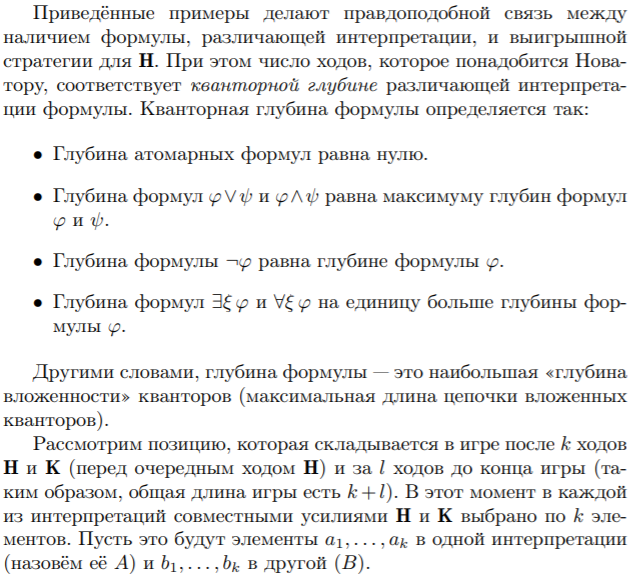
\includegraphics[width=0.48\textwidth]{images/1.14_страница1.PNG}
    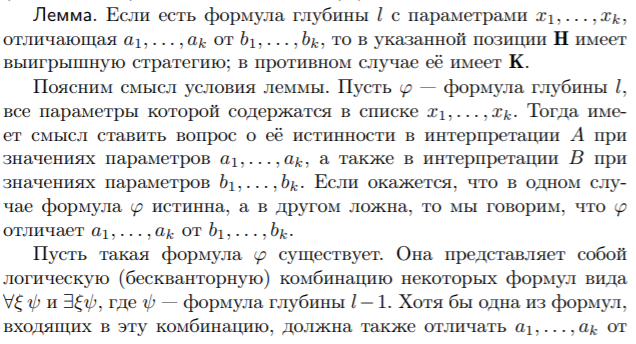
\includegraphics[width=0.48\textwidth]{images/1.14_страница2.PNG}

    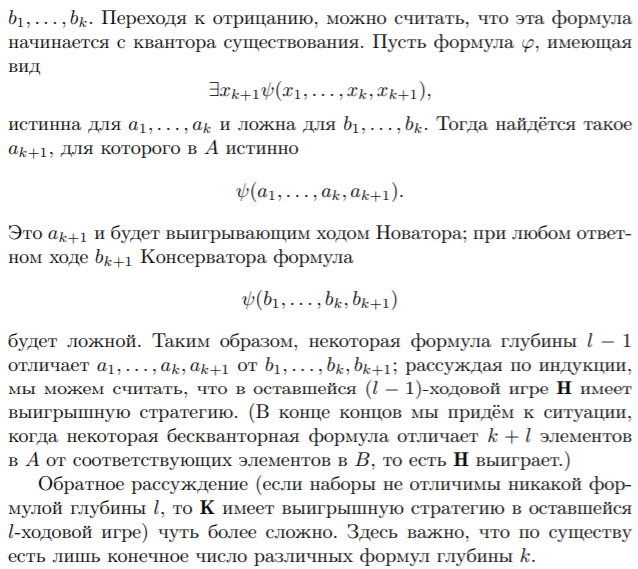
\includegraphics[width=0.48\textwidth]{images/1.14_страница3.PNG}
    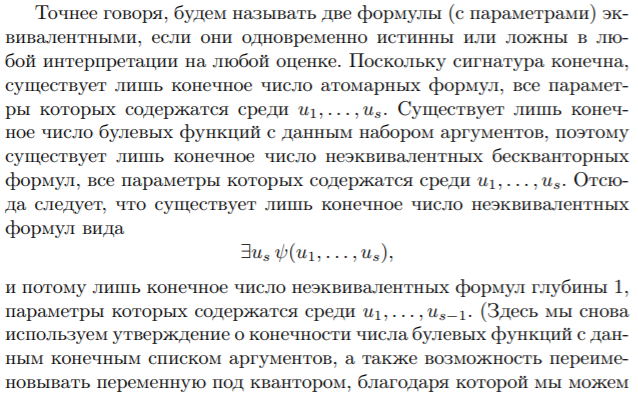
\includegraphics[width=0.48\textwidth]{images/1.14_страница4.PNG}

    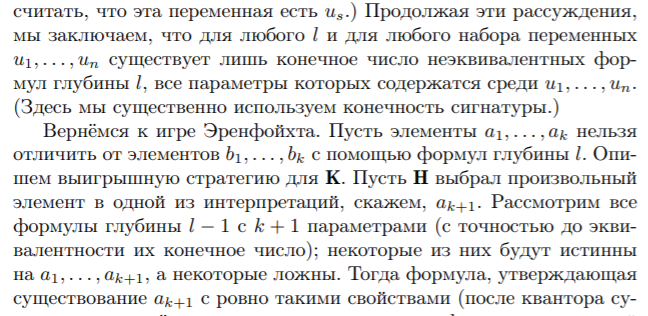
\includegraphics[width=0.48\textwidth]{images/1.14_страница5.PNG}
    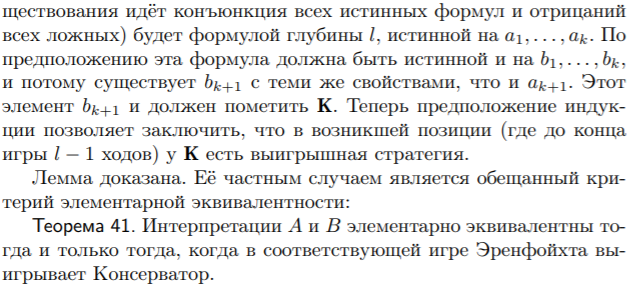
\includegraphics[width=0.48\textwidth]{images/1.14_страница6.PNG}
\end{center}

\textbf{Теорема.} Теорема Эренфойхта 

Две интерпретации элементарно эквивалентны $\Leftrightarrow$ в соответсвующей игре побеждает Консерватор.

\textbf{Утверждение.} Упорядоченные множества $\mathbb{Z}$ и $\mathbb{Z} + \mathbb{Z}$  элементарно эквивалентны.

Доказывается через игру Эренфойхта. В данном примере важно, что Новатор заранее ограничивает число своих ходов.

(Идея нетривиальная. Но думаю, что на экзамене не составит труда самостоятельно придумать стратегию для Консерватора.)

\textbf{Идея (от Мусатова):}  Консерватор не отличает бесконечные отрезки (отрезки, у которых концы находятся в разных множествах $\mathbb{Z}$) от "очень длинных" (определены ниже). Поддерживает некоторый инвариант: порядок на отмеченных элементах один и тот же, расстояния между соответствующими элементами либо маленькие и одинаковые, либо большие. В конце игры важен только порядок, так что если Консерватору удастся поддерживать этот инвариант, то он выиграет.\\
За $m$ раундов до конца будем называть "очень длинным" любой отрезок длины $\geq 2^m$. Если Новатор отмечает точку внутри очень длинного длинного отрезка, то из образованных (делением отрезка точкой) отрезков хотя бы один тоже будет очень длинным на следующей стадии (когда $m$ на $1$ меньше). Действительно, если каждый из них короче $2^{m-1}$, то изначальный был бы короче $2^m$. В любом случае Консерватор сможет повторить этот ход: либо с одной стороны образовать короткий отрезок той же длины, либо разделить на два очень длинных. Если Новатор отмечает точку внутри короткого отрезка, то Консерватор сможет повторить такой ход. В любом случае Консерватор сможет поддержать инвариант. Следовательно, Консерватор победит. Следовательно, упорядоченные множества $\mathbb{Z}$ и $\mathbb{Z} + \mathbb{Z}$ элементарно эквивалентны.

\textbf{Стратегия для Консерватора от автора конспекта:} 

Первый ход Консерватор делает как угодно.

Путь было сделано $n$ ходов. В одном множестве отмечены элементы $a_1, \ldots, a_n$, в другом $b_1, \ldots, b_n$, причём $\forall i \ a_i$ соответствует $b_i$ и $a_i < a_{i + 1}$, соответственно $b_i < b_{i + 1}$. Новатор выбирает элемент $k$ между $a_i$ и $a_{i + 1}$ (Не важно $[a_i, a_{i + 1}]$ конечный или бесконечный). Если отрезок $[b_i, b_{i + 1}]$ конечный, то консерватор отмечает элемент в середине этого отрезка. Если отрезок $[b_i, b_{i + 1}]$ бесконечный, то консерватор отмечает любую точку между $b_i$ и $b_{i + 1}$. Порядок сохранился. Сделаем перенумерацию и переходим к следующему шагу. Так как между любыми двумя отмеченными объектами континуальное или бесконечное количество точек, то Консерватор в любом случае сможет поддержать инвариант. Следовательно, Консерватор победит. Следовательно, упорядоченные множества $\mathbb{Z}$ и $\mathbb{Z} + \mathbb{Z}$ элементарно эквивалентны. 